
\section{三个例子}

我们现在给出三个篇幅较长的例子。短期目标是看到：我们确实能够驾驭\trStructureSheaf，并能对有趣的%
\trOpenSet{}算出其\trSection{}环——这些\trOpenSet{}不再只是\trAffineScheme{}的\trDistinguishedOpen。%
长期目标是遇见一些有趣的例子，它们将在日后反复登场。

\textbf{4.4.1.\ 第一个例子：挖去原点的（\trAffine）平面。}\quad 这个例子将让你看到：\trDistinguishedBase{}%
是一种你真正能够上手的东西。设 $A=k[x,y]$，于是 $\Spec A=\mathbb{A}^2_k$。我们来把\trOpenSet{}%
$U=\mathbb{A}^2\smallsetminus\{(0,0)\}=\mathbb{A}^2\smallsetminus\{[(x,y)]\}$ 上的函数空间算出来。

这是不是一个\trDistinguishedOpen，并非一目了然。（事实上它不是——哪怕你现在还看不出来，%
再过几段你多半就能想明白缘由。仅证明 $(x,y)$ 不是\trPrincipalIdeal{}是不够的。）但无论如何，我们可以把它%
描述为两个\emph{确实}是\trDistinguishedOpen{}的东西之并：$U=D(x)\cup D(y)$。我们将把 $D(x)$ 上的%
函数与 $D(y)$ 上的函数粘合起来，从而找出 $U$ 上的函数。

根据\cref{thm:structure-sheaf-definition}，$D(x)$ 上的函数是 $A_x=k[x,y,1/x]$；$D(y)$ 上的函数是%
$A_y=k[x,y,1/y]$。注意：$A$ \trInjectiveMap{}到它的诸\trLocalization{}之中（只要不让 $0$ 被取逆），%
因为它是\trIntegralDomain（\cref{ex:when-localization-is-injective}）；于是 $A$ \trInjectiveMap{}入%
$A_x$ 与 $A_y$ 二者，而这两者又都\trInjectiveMap{}入 $A_{xy}$（而且确实\trInjectiveMap{}入%
$k(x,y)=K(A)$）。于是，我们要找的是 $D(x)$ 与 $D(y)$ 上在 $D(x)\cap D(y)=D(xy)$ 处相互一致的%
函数；换言之，我们是在 $A_{xy}$（或在 $k(x,y)$）中解读 $A_x\cap A_y$。显然，那些分母中只有 $x$ 的幂、%
同时又只有 $y$ 的幂的\trRationalFunction{}就是多项式。「翻译」过来即：$A_x\cap A_y=A$。%
于是我们得出结论：
\begin{equation*}\tag{4.4.1.1}\label{eq:global-sections-plane-minus-origin}
\Gamma(U,\OO_{\mathbb{A}^2})=k[x,y].
\end{equation*}
换言之，挖去原点并没有给我们带来任何额外的函数。注意这一计算是何等轻松！

\textbf{4.4.2.\ 题外话。}\quad 注意：$\mathbb{A}^2\smallsetminus\{(0,0)\}$ 上的任何函数都可以延拓到%
整个 $\mathbb{A}^2$ 之上。这是\trComplexGeometry{}中\trHartogs{}引理（Hartogs's Lemma）的一个类似物：%
在\trComplex\trManifold{}上，定义在\trCodimension{}至少为 $2$ 的\trSet{}的\trComplement{}上的\trHolomorphic{}函数，%
可以越过这缺失的集合延拓出去。在代数的背景里，这件事将在更一般的情形成立：\trCodimension{}至少为 $2$ 的点，%
不仅当它们「\trSmooth」时可以被越过，而且当它们轻度奇异时也可以——我们日后将把这种性质称为%
\emph{\trNormal}（normal）。我们将在 \S13.5.19 中把这一点说精确。这个事实对我们将会非常有用。

\textbf{4.4.3.}\quad 我们现在展示一个有趣的事实：$(U,\OO_{\mathbb{A}^2}|_U)$ 是一个\trScheme，%
但它不是\trAffineScheme。（这一点容易让人犯迷糊，所以你得打起精神。）缘由如下：否则，%
若 $(U,\OO_{\mathbb{A}^2}|_U)\cong(\Spec A',\OO_{\Spec A'})$，那么取\trGlobalSections{}便可复原 $A'$：
\[
A'=\Gamma(U,\OO_{\mathbb{A}^2}|_U),
\]
而我们已在 \eqref{eq:global-sections-plane-minus-origin} 中把它认同为 $k[x,y]$。于是若 $U$ 是\trAffine{}的，%
我们就有\trIsomorphism
\[
U\overset{\sim}{\longrightarrow}\Spec A'=\Spec k[x,y]=\mathbb{A}^2_k.
\]
但是，环中\trPrimeIdeal{}与谱的点之间的这个\trBijection，其实比表面看来的更具构造性：%
\emph{给了\trPrimeIdeal{} $I$，%
你可以把这个点复原为由 $I$ 割出的\trClosedSubset{}的\trGenericPoint，即 $V(I)$；而给了点 $\mathfrak{p}$，%
你可以把理想复原为在 $\mathfrak{p}$ 处消失的那些函数，即 $I(\mathfrak{p})$。}特别地，$A'$ 的%
\trPrimeIdeal{} $(x,y)$ 应当在 $\Spec A'$ 中割出一个点。但在 $U$ 上，$V(x)\cap V(y)=\varnothing$。%
结论：$U$ \emph{不是}\trAffineScheme。（日后你若要找某件事的反例，而且预计反例会涉及一个非\trAffineScheme，%
请把这个例子记在心上！）

\textbf{4.4.4.\ 用两种不同的方式把两份 $\mathbb{A}^1$ 粘合起来。}\quad 至今我们已见过非\trAffineScheme{}的%
两个例子：非空\trScheme{}的无穷\trDisjointUnion（\cref{ex:disjoint-union-schemes}），以及 $\mathbb{A}^2\smallsetminus\{(0,0)\}$。%
我想再给你两个例子。它们很重要，因为它们是最早展现基本行为的例子——第一个是病态的，第二个则是核心的。

首先，我得告诉你如何把两个\trScheme{}粘合起来。在此之前，你应当复习一下如何沿同构的\trOpenSet{}粘合两个%
\trTopologicalSpace。给定两个\trTopologicalSpace{} $X$ 与 $Y$，以及\trOpenSubset{} $U\subset X$ 与%
$V\subset Y$，连同\trHomeomorphism{} $U\overset{\sim}{\longrightarrow}V$，我们就能造出一个新的%
\trTopologicalSpace{} $W$，我们把它想成是沿 $U\overset{\sim}{\longrightarrow}V$ 把 $X$ 与 $Y$ 粘合起来的%
产物。它是不交并 $X\sqcup Y$ 关于\trEquivalenceRelation{} $U\sim V$ 的\trQuotient，其中商被赋予\trQuotientTopology{}。%
于是 $X$ 与 $Y$ 自然地（被认同为）$W$ 的\trOpenSubset，而且确实\trCover{}住 $W$。%
你能对任意（不必有限）多个\trTopologicalSpace，%
把这番叙述干净利落地重述一遍吗？

讨论完\trTopologicalSpace{}的粘合，现在来粘合\trScheme。（对更一般的\trRingedSpace，这套做法也原封不动地%
适用。）设你有两个\trScheme{} $(X,\OO_X)$ 与 $(Y,\OO_Y)$，以及\trOpenSubset{} $U\subset X$ 与 $V\subset Y$，%
连同\trHomeomorphism{} $\pi\colon U\overset{\sim}{\longrightarrow}V$，以及诸\trStructureSheaf{}的一个%
\trIsomorphism{} $\OO_V\overset{\sim}{\longrightarrow}\pi_*\OO_U$（也就是说，\emph{\trScheme}的%
\trIsomorphism{} $(U,\OO_X|_U)\overset{\sim}{\longrightarrow}(V,\OO_Y|_V)$）。那么我们就能把它们粘合起来，%
得到单个\trScheme。理由：设 $W$ 是用\trIsomorphism{} $U\overset{\sim}{\longrightarrow}V$ 把 $X$ 与 $Y$ 粘合%
所得。则\cref{ex:gluing-sheaves-cocycle}表明，诸\trStructureSheaf{}可以粘合起来得到一个\trRing{}的\trSheaf。%
注意这确实是一个\trScheme：任何一点都有某个作为\trAffineScheme{}的\trNeighborhood。（你看出缘由了吗？）

\begin{exercise}[必要练习，对照\cref{ex:gluing-sheaves-cocycle}]\label{ex:glue-arbitrary-schemes}
证明你可以把任意一族\trScheme{}粘合起来。设给定如下数据：
\begin{itemize}
\item \trScheme{} $X_i$（$i$ 跑遍某个\trIndexSet{} $I$，不必有限）；
\item \trOpenSubscheme{} $X_{ij}\subset X_i$，满足 $X_{ii}=X_i$；
\item \trIsomorphism{} $f_{ij}\colon X_{ij}\overset{\sim}{\longrightarrow}X_{ji}$，
      其中 $f_{ii}$ 为\trIdMorphism，
\end{itemize}
使得
\begin{itemize}
\item （\trCocycleCondition）诸\trIsomorphism{}「在三重交上一致」，即%
$f_{ik}\big|_{X_{ij}\cap X_{ik}}=f_{jk}\big|_{X_{ji}\cap X_{jk}}\circ f_{ij}\big|_{X_{ij}\cap X_{ik}}$%
（于是，不言自明地，为使右边有意义，需要 $f_{ij}(X_{ik}\cap X_{ij})\subset X_{jk}$）。
\end{itemize}
（\trCocycleCondition{}保证 $f_{ij}$ 与 $f_{ji}$ 互为逆。事实上，「$f_{ii}$ 为\trIdMorphism」这一假设%
也可由\trCocycleCondition{}推出。）证明：存在唯一的\trScheme{} $X$（在相差唯一\trIsomorphism{}的意义下），%
连同与诸 $X_i$ \trIsomorphic{}的\trOpenSubscheme{}，它们以显而易见的方式尊重这份粘合数据。%
（提示：作为\trSet，$X$ 是什么？这个\trSet{}上的\trTopology{}是什么？%
按照你对 $X$ 诸\trOpenSet{}的描述，这个\trSheaf{}在%
每个\trOpenSet{}上的\trSection{}是什么？）你或许愿意通过描述 $X$ 所满足的一个\trUniversalProperty{}%
来证明唯一性（在相差唯一\trIsomorphism{}的意义下）。
\end{exercise}

现在我就给你两个非\trAffineScheme。它们都值得熟记于心。两种情形下，我都会把\trAffineLine{} $\mathbb{A}^1_k$%
的两份副本粘合起来。设 $X=\Spec k[t]$，$Y=\Spec k[u]$。设 $U=D(t)=\Spec k[t,1/t]\subset X$ 与%
$V=D(u)=\Spec k[u,1/u]\subset Y$。两个例子都将由沿 $U$ 与 $V$ 粘合 $X$ 与 $Y$ 而得；差别只在怎么粘。

\textbf{4.4.5.\ 第二个例子：原点加倍了的\trAffineLine。}\quad 考虑经由\trIsomorphism{}%
$k[t,1/t]\overset{\sim}{\longrightarrow}k[u,1/u]$（由 $t\longleftrightarrow u$ 给出；对照\cref{ex:scheme-isos-ring-isos}）%
而来的 $U\overset{\sim}{\longrightarrow}V$。所得的\trScheme{}称为\textbf{原点加倍了的\trAffineLine}%
（affine line with doubled origin）。图~\ref{fig:affine-line-doubled-origin}是它的一幅图。

\begin{figure}[htbp]
\centering
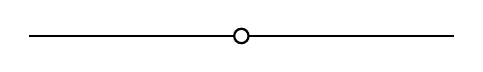
\begin{tikzpicture}[scale=1.0]
  \draw[thick] (-2.7,0) -- (2.7,0);
  \draw[thick,fill=white] (0,0) circle (2.6pt);
\end{tikzpicture}
\caption{原点加倍了的\trAffineLine{}。（依原书手绘图重绘。）}%
\label{fig:affine-line-doubled-origin}
\end{figure}

正如图画所暗示的，直观上这是\trHausdorff{}性质失效的一个类比。当然，$\mathbb{A}^1$ 本身并不是%
\trHausdorff{}的，所以我们不能说它是\trHausdorff{}性质的失效。我们觉得这事又古怪又糟糕，%
因此我们会想造出一个定义来防止这类事情发生。这将是\emph{\trSeparatedness}（separatedness）的观念%
（将在第~11~章中讨论）。（事实上，在某种意义上，\trSeparatedness{}才是\trHausdorff{}性质\emph{正确}的%
定义；见练习~11.2.B！）它还将应验我们在别处的祈祷。例如，在\trSeparated{}\trScheme{}上，%
「\trZariskiTopology{}的\trAffine\trBase」十分良好——两个\trAffine\trOpenSet{}的交将是\trAffine{}的%
（命题~11.2.13）。

\begin{exercise}\label{ex:doubled-origin-line-not-affine}
证明原点加倍了的\trAffineLine{}不是\trAffine{}的。提示：算出\trGlobalSections{}环，并回头看看关于%
$\mathbb{A}^2\smallsetminus\{(0,0)\}$ 的那个论证。
\end{exercise}

\begin{exercise}[容易的练习]\label{ex:doubled-origin-plane}
把同一构造中的 $\mathbb{A}^1$ 换成 $\mathbb{A}^2$ 再做一遍。你将定义出\textbf{原点加倍了的\trAffine{}平面}%
（affine plane with doubled origin）。描述这个\trScheme{}的两个\trAffine\trOpenSubset，使其交不是一个%
\trAffine\trOpenSubset。（这个例子已在警示~4.3.3 中被许诺。此外，「无穷维」版本将出现在练习~5.1.K 中。）
\end{exercise}

\textbf{4.4.6.\ 第三个例子：\trProjectiveLine{}。}\quad 考虑经由 $t\leftrightarrow 1/u$ 给出的\trIsomorphism{}%
$k[t,1/t]\overset{\sim}{\longrightarrow}k[u,1/u]$ 而来的 $U\cong V$。图~\ref{fig:gluing-p1}是这次粘合的%
一幅富有启发性的图。所得的\trScheme{}称为\textbf{\trField{} $k$ 上的\trProjectiveLine{}}%
（projective line over the field $k$），记作 $\mathbb{P}^1_k$。

\begin{figure}[htbp]
\centering
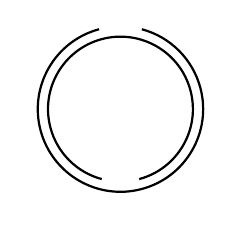
\begin{tikzpicture}[scale=1.0,line width=0.8pt]
  \draw (105:1.05) arc (105:435:1.05);
  \draw (285:0.92) arc (285:615:0.92);
\end{tikzpicture}
\caption{把两条\trAffineLine{}粘合起来得到 $\mathbb{P}^1$。（依原书手绘图重绘。）}%
\label{fig:gluing-p1}
\end{figure}

注意这些点是怎样粘合的。为方便起见，让我假设 $k$ 是\trAlgClosed{}的。（你可以想一想，若不然%
情况会如何改变。）在第一条\trAffineLine{}上，我们有闭的（「传统的」）点 $[(t-a)]$，我们把它想成%
「$t$-直线上的 $a$」，还有\trGenericPoint{} $[(0)]$。在第二条\trAffineLine{}上，我们有%
「$u$-直线上的 $b$」这样的\trClosedPoint，以及\trGenericPoint。于是，$t$-直线上的 $a$ 被粘到%
$u$-直线上的 $1/a$（当然，要求 $a\neq 0$），而\trGenericPoint{}被粘到\trGenericPoint（$k[t]$ 的%
\trIdeal{} $(0)$ 经\trLocalization{}后成为 $k[t,1/t]$ 的\trIdeal{} $(0)$，$k[u]$ 的\trIdeal{} $(0)$%
经\trLocalization{}后成为 $k[u,1/u]$ 的\trIdeal{} $(0)$；而在\trIsomorphism{} $t\longleftrightarrow 1/u$
之下，$k[t,1/t]$ 中的 $(0)$ 就是 $k[u,1/u]$ 中的 $(0)$）。

\textbf{4.4.7.}\quad 若 $k$ 是\trAlgClosed{}的，我们可以按下述方式解读 $\mathbb{P}^1_k$ 的%
\trClosedPoint{}——这也许会让你觉得，它更接近你先前见过的\trProjectiveSpace{}的定义方式。%
这些点形如 $[a,b]$，其中 $a$ 与 $b$ 不全为零，且 $[a,b]$ 被认同于 $[ac,bc]$，其中 $c\in k^{\times}$。%
那么，当 $b\neq 0$ 时，它被认同于 $t$-直线上的 $a/b$；当 $a\neq 0$ 时，它被认同于 $u$-直线上的 $b/a$。

\vkthmsync{8}
\begin{proposition}\label{thm:p1-not-affine}
$\mathbb{P}^1_k$ \emph{不是\trAffine{}的}。
\end{proposition}

\emph{证明。}\ 我们通过计算\trGlobalSections{}环来证明。\trGlobalSections{}对应于 $X$ 上的\trSection{}%
与 $Y$ 上的\trSection{}中在重叠处相互一致的那些。$X$ 上的一个\trSection{}是多项式 $f(t)$；%
$Y$ 上的一个\trSection{}是多项式 $g(u)$。把 $f(t)$ 限制到重叠上，得到的那个东西仍可称之为 $f(t)$；%
对 $g(u)$ 亦然。现在我们要求二者相等：$f(t)=g(1/t)$。但既是 $t$ 的多项式又是 $1/t$ 的多项式者，%
只有常值 $k$。于是 $\Gamma(\mathbb{P}^1,\OO_{\mathbb{P}^1})=k$。若 $\mathbb{P}^1$ 是\trAffine{}的，%
则它将是 $\Spec\Gamma(\mathbb{P}^1,\OO_{\mathbb{P}^1})=\Spec k$，也就是说，一个点。但它不是——%
它有许许多多的点。\hfill$\square$

我们由此证明了一条重要定理的类比：$\mathbb{CP}^1$ 上的\trHolomorphic{}函数只有常值函数！%
（关于一个严肃却又容易的推广，见 \S11.4.7。）

\textbf{4.4.9.\ 重要例子：\trProjectiveSpace。}\quad 我们现在给出\textbf{\trField{} $k$ 上的\trProjective{} $n$-空间}%
（projective $n$-space over a field $k$）的一个初步定义，记作 $\mathbb{P}^n_k$：把 $n+1$ 个%
\trOpenSet{}粘合起来，其中每一个都\trIsomorphic{}于 $\mathbb{A}^n_k$。为这些\trOpenSet{}择取明智的%
记号，会让我们的日子好过些。动机如下。在上述 $\mathbb{P}^1$ 的构造中，我们把\trProjectiveSpace{}的点%
想成 $[x_0,x_1]$，其中 $(x_0,x_1)$ 只在相差标量的意义下确定，即 $(x_0,x_1)$ 与%
$(\lambda x_0,\lambda x_1)$ 被视为相同。于是，第一张「卡」（patch）可以解读为：取 $x_0\neq 0$ 的%
那个\trLocus，然后考虑点 $[1,t]$，并把 $t$ 想成 $x_1/x_0$；尽管 $x_0$ 与 $x_1$ 都不是\trWellDefined{}的，%
$x_1/x_0$ 却是。第二张「卡」对应于 $x_1\neq 0$ 的情形：我们考虑点 $[u,1]$，并把 $u$ 想成 $x_0/x_1$。%
改用记号 $x_{1/0}$ 表示 $t$、$x_{0/1}$ 表示 $u$，将会很有用。

对 $\mathbb{P}^n$，我们把 $n+1$ 个\trOpenSet{}粘合起来，$i=0,\dots,n$ 各取其一。第 $i$ 个%
\trOpenSet{} $U_i$ 将具有坐标 $x_{0/i}$、……、$x_{(i-1)/i}$、$x_{(i+1)/i}$、……、$x_{n/i}$。%
采用写法
\begin{equation*}\tag{4.4.9.1}\label{eq:proj-patches-notation}
\Spec k[x_{0/i},x_{1/i},\dots,x_{n/i}]/(x_{i/i}-1)
\end{equation*}
会很方便。（这样我们引入了一个「哑变量」$x_{i/i}$，随即就把它取值为 $1$。）我们把 $U_i$ 的%
\trDistinguishedOpen{} $D(x_{j/i})$ 粘合到 $U_j$ 的\trDistinguishedOpen{} $D(x_{i/j})$ 上，办法是%
描述环的认同，从而认同这两个\trScheme：
\[
\begin{aligned}
&k[x_{0/i},x_{1/i},\dots,x_{n/i},1/x_{j/i}]/(x_{i/i}-1)\\
&\qquad\cong k[x_{0/j},x_{1/j},\dots,x_{n/j},1/x_{i/j}]/(x_{j/j}-1)
\end{aligned}
\]
认同方式为 $x_{k/i}=x_{k/j}/x_{i/j}$、$x_{k/j}=x_{k/i}/x_{j/i}$（这蕴涵 $x_{i/j}x_{j/i}=1$）。%
我们还需要检验：这份粘合信息在三重重叠处是相容的。

\begin{exercise}\label{ex:proj-triple-overlap}
尽可能不痛地检验这件事。（可能的提示：三重交是\trAffine{}的；请描述相应的环。）
\end{exercise}

\vkthmsync{10}
\begin{definition}[$\mathbb{P}^n_A$]\label{thm:projective-space-over-ring}
注意，我们的定义并未用到 $k$ 是\trField{}这一事实。因此，我们不妨对任意\emph{\trRing} $A$ 定义%
$\mathbb{P}^n_A$。这日后会派上用场。
\end{definition}

\begin{exercise}\label{ex:proj-functions-constant}
证明 $\mathbb{P}^n_k$ 上的函数只有常值函数（$\Gamma(\mathbb{P}^n_k,\OO)\cong k$），从而当 $n>0$ 时%
$\mathbb{P}^n_k$ 不是\trAffine{}的。提示：你也许会担心，需要在你的全部\trAffine\trOpenSet{}之间作某种精巧的%
相互配合；但其实，只需其中两个\trOpenSet{}便能看出这件事。这背后甚至还有几何直观：%
两个\trOpenSet{}之并的\trComplement{}\trCodimension{}为 $2$。而「\trAlgebraic{}\trHartogs{}引理」%
（在 \S4.4.2 中被非正式地讨论过，并将在定理~13.5.19 中得到严格陈述）说：定义在这个并上的任何函数%
都可延拓为整个\trProjectiveSpace{}上的函数。既然我们预期\trProjectiveSpace{}上的函数只有常值函数，%
那么在我们这两个\trAffine\trOpenSet{}的并上，这一点就应当已经显现了。
\end{exercise}

\begin{exercise}[推广 \S4.4.7]\label{ex:closed-points-pn-traditional}
证明：若 $k$ 是\trAlgClosed{}的，则 $\mathbb{P}^n_k$ 的\trClosedPoint{}可以按传统方式解读：%
点形如 $[a_0,\dots,a_n]$，其中诸 $a_i$ 不全为零，且 $[a_0,\dots,a_n]$ 被认同于%
$[\lambda a_0,\dots,\lambda a_n]$，其中 $\lambda\in k^{\times}$。
\end{exercise}

有益的翻译：我们把 $\mathbb{P}^n_k$（其中 $k=\overline{k}$）的\trClosedPoint{}想成%
$[x_0,x_1,\dots,x_n]$，其中 $x_i\in k$（诸 $x_i$ 不全为零），并对一切 $\lambda\in k^{\times}$ 把%
$[x_0,x_1,\dots,x_n]$ 认同于 $[\lambda x_0,\lambda x_1,\dots,\lambda x_n]$。于是，%
$[x_0,x_1,\dots,x_n]$ 对应于一条过原点的直线，而 $(x_{0/i},x_{1/i},\dots,x_{n/i})$ 就是这条直线与%
\trHyperplane{} $x_i=1$ 相交之处。

我们日后会给出\trProjectiveSpace{}的其他定义（定义~4.5.9、\S15.2.3），届时诸 $x_i$ 将被称为%
\emph{\trProjective{}坐标}（projective coordinates）。我们在这里给出的第一个定义，做起计算来常常很顺手；%
但它有些不自然之处——\trProjectiveSpace{}是高度对称的，而从我们目前的定义里看不出这一点。%
此外，正如H.~\trWeyl（[Wey, p.~90]）所指出的：「把数作为坐标引入，是一种暴力行为。」

\textbf{4.4.11.\ 有趣的题外话：\trChineseRemainderTheorem{}是一个\emph{几何}事实。}\quad \trChineseRemainderTheorem{}就嵌在我们%
做过的事情之中。我们将通过一个单独的例子看到这一点，但你随后应当把一般陈述自己想明白。%
\trChineseRemainderTheorem{}说：知道一个整数模 $60$ 的余数，与知道它模 $3$、$4$ 与 $5$ 的余数，是一回事。%
下面是用\trScheme{}的语言来看这件事的方式。$\Spec\mathbb{Z}/(60)$ 是什么？这个\trRing{}的\trPrimeIdeal{}%
有哪些？答：$\mathbb{Z}$ 中包含 $(60)$ 的那些\trPrimeIdeal，也就是整除 $60$ 的那些素数，%
即 $(2)$、$(3)$ 与 $(5)$。图~\ref{fig:spec-z-60}是 $\Spec\mathbb{Z}/(60)$ 的一幅草图。%
它们都是\trClosedPoint，因为这些都是\trMaximalIdeal，于是其\trTopology{}是\trDiscreteTopology。%
\trStalk{}是什么？你可以验证：它们是 $\mathbb{Z}/(4)$、$\mathbb{Z}/(3)$ 与 $\mathbb{Z}/(5)$。%
「在 $(2)$ 处」的\trNilpotent{}元由该点上的「\trFuzz{}」标示。（\S4.2 中我们讨论过用%
「无穷小\trFuzz{}」可视化\trNilpotent{}元。）那么这个\trScheme{}上的\trGlobalSections{}是什么？%
它们是「这个\trOpenSet{} $(2)$」「另一个\trOpenSet{} $(3)$」与「第三个\trOpenSet{} $(5)$」上的%
\trSection。换言之，我们有环的一个\trNaturalIsomorphism
\[
\mathbb{Z}/(60)\overset{\sim}{\longrightarrow}\mathbb{Z}/(2^2)\times\mathbb{Z}/(3)\times\mathbb{Z}/(5).
\]

\begin{figure}[htbp]
\centering
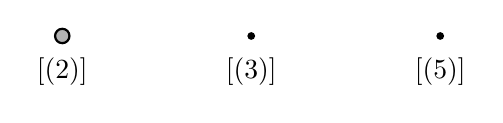
\begin{tikzpicture}[scale=1.0]
  \filldraw[fill=gray!60,line width=0.8pt] (0,0) circle (2.6pt);
  \fill (2.4,0) circle (1.4pt);
  \fill (4.8,0) circle (1.4pt);
  \node at (0,-0.45) {$[(2)]$};
  \node at (2.4,-0.45) {$[(3)]$};
  \node at (4.8,-0.45) {$[(5)]$};
\end{tikzpicture}
\caption{$\Spec\mathbb{Z}/(60)$ 的一幅图。（依原书手绘图重绘。）}%
\label{fig:spec-z-60}
\end{figure}

\vkthmsync{12}
\begin{example}[\extrahard]\label{thm:quadric-cone-section-example}
这是\trScheme{}的某个\trOpenSubset{}上一个函数的例子，其行为有些出人意料。在%
$X=\Spec k[w,x,y,z]/(wz-xy)$ 上考虑\trOpenSubset{} $D(y)\cup D(w)$。显然，$D(y)$ 上的函数 $z/y$ 与%
$D(w)$ 上的函数 $x/w$ 在重叠 $D(y)\cap D(w)$ 上一致。于是它们粘合起来给出一个\trSection。%
在\trComplexGeometry{}中思考\trAnalytic{}延拓（analytic continuation）时，你也许见过这种局面——我们有一个%
「\trHolomorphic{}」函数，它在某个\trOpenSet{}上由 $z/y$ 描述，而这个描述在别处失效，但你仍可以通过让这个%
函数在空间的不同部分取不同的定义，来对它进行「\trAnalytic{}延拓」。
\end{example}

\emph{给好奇行家的后续讨论。}\ 这个函数没有任何用 $w$、$x$、$y$、$z$ 表出的「单一描述」可以成为%
\trWellDefined{}的表达式！这里有大量有趣的几何，而这个\trScheme{}将是我们取之不竭的（反）例来源%
（在索引中查「反复登场的（反）例」）。下面用它尚未定义的语言，先给你惊鸿一瞥。空间%
$\Spec k[w,x,y,z]$ 是 $\mathbb{A}^4$，不出所料，是四维的。我们打交道的对象是子集 $X$，它是一张%
\trHypersurface，是三维的。它是 $\mathbb{P}^3$ 中一张\trSmooth\trQuadricSurface{}上的\trCone%
（翻到图~9.2）。\trOpenSubset{} $D(y)\subset X$ 是 $X$ 减去某张\trHypersurface，所以我们扔掉的%
是一个\trCodimension{} $1$ 的\trLocus。\trOpenSubset{} $D(w)$ 则还要扔掉另一个\trCodimension{} $1$ 的\trLocus。%
你也许会想：这两块被丢弃的\trLocus{}之交于是\trCodimension{}为 $2$，而这个古怪函数之所以不能延拓为%
整体多项式，是因为我们那条\trHartogs{}引理型的定理失效了。但事实并非如此——%
$V(y)\cap V(w)$ 其实\trCodimension{}为 $1$。实际发生的情况如下。空间 $V(y)$ 的得到方式，是扔掉%
（两条直线 $\ell$ 与 $m_1$ 之并上的）\trCone，这两条直线在\trSurface{}的两族「\trRuling{}」（ruling）中各居其一；\footnote{译注：此处原文作 $V(y)$；按数学内容，如此「扔掉锥」所得的空间应为 $D(y)$。}%
$V(w)$ 同样涉及扔掉（两条直线 $\ell$ 与 $m_2$ 之并上的）\trCone。其交是（直线 $\ell$ 上的）\trCone，%
这是一个\trCodimension{} $1$ 的\trSet。令人称奇的是：尽管它是「纯\trCodimension{} $1$」的，$\ell$ 上的这个\trCone{}却%
连作为\trSet{}都无法由单个方程割出（见练习~15.5.N）。这意味着：对我们的函数而言，任何形如%
$f(w,x,y,z)/g(w,x,y,z)$ 的表达式都不能正确描述它在 $D(y)\cup D(w)$ 上的取值——在%
$D(y)\cup D(w)$ 的某一点处，它必定是 $0/0$。缘由如下。我们的函数无法定义在 $V(y)\cap V(w)$ 上，%
所以 $g$ 必须在这里消失。但 $g$ 不能只在 $\ell$ 上的\trCone{}处消失——它必须在别处也消失。
